\documentclass[conference]{IEEEtran}
\IEEEoverridecommandlockouts
\usepackage{cite}
\usepackage{amsmath,amssymb,amsfonts}
\usepackage{algorithmic}
\usepackage{graphicx}
\usepackage{textcomp}
\usepackage{xcolor}
\usepackage{adjustbox} % For resizing tables
\def\BibTeX{{\rm B\kern-.05em{\sc i\kern-.025em b}\kern-.08em
    T\kern-.1667em\lower.7ex\hbox{E}\kern-.125emX}}
\begin{document}

\title{From Indoor Prototypes to Robust Outdoor Autonomy: A Comprehensive Analysis of State-of-the-Art SLAM Algorithms and Insights for Large-Scale Environments}

\author{\IEEEauthorblockN{Muhammad Zeeshan Asghar}
\IEEEauthorblockA{\textit{Faculty of Computer Science} \\
\textit{HSE University}, Moscow, Russia}
}

\maketitle

\begin{abstract}
Simultaneous Localization and Mapping (SLAM) is central to autonomous navigation, enabling agents such as self-driving cars, drones, and field robots to build maps of unknown areas while estimating their trajectories on the fly. Initially formulated for controlled indoor scenarios, SLAM research has expanded to address the more complex, large-scale outdoor domains that characterize real-world applications. These outdoor scenarios introduce a host of challenges, including extended operational ranges, sparse or repetitive features, dynamic moving objects, varying illumination, and unpredictable weather conditions.

This survey presents a thoroughly analyzed perspective on the evolution of SLAM from indoor proofs-of-concept to robust large-scale outdoor operations. Emphasizing depth and clarity, we spotlight a small number of highly cited, state-of-the-art methods—such as ORB-SLAM2, LOAM, and VINS-Fusion—and dissect their algorithmic foundations, optimization frameworks, sensor fusion techniques, and strategies for handling dynamics. We highlight foundational works like ORB-SLAM2, LOAM, and VINS-Fusion that established performance benchmarks, as well as advanced paradigms such as direct visual methods (LSD-SLAM, DSO), semantic and dynamic-scene approaches (DynaSLAM), and learning-driven pipelines (SuperGlue, DeepVO).

Throughout this survey, we emphasize not just what these algorithms do, but the key ideas and insights that guided their design choices—why certain feature detectors, factor graph formulations, or sensor integrations were chosen, and how these decisions overcome the hurdles of large-scale outdoor domains. We integrate a comparative table summarizing methods’ characteristics and present five example figures (with pointers to their original sources), ensuring clarity and multi-faceted analysis. In concluding, we discuss persistent challenges—dynamic scenes, long-term mapping, environmental adaptation, and scalability—and identify promising future directions that build on the lessons distilled here.
\end{abstract}

\begin{IEEEkeywords}
SLAM, large-scale outdoor environments, factor graphs, ORB-SLAM2, LOAM, VINS-Fusion, direct SLAM, semantic SLAM, multi-sensor fusion, deep learning.
\end{IEEEkeywords}

\section{Introduction}
Simultaneous Localization and Mapping (SLAM) solves a key puzzle in robotics and autonomous systems: how can an agent navigate an unknown environment while simultaneously constructing a map of it? Initially, SLAM was developed and tested in small, controlled indoor scenarios—like corridors or labs—where the complexity of scale, variability, and dynamics was limited. However, real-world applications increasingly demand robust autonomous navigation in large-scale outdoor domains: cars driving through sprawling cities, drones scanning miles of farmland, and rovers exploring remote terrains.

These outdoor settings stress SLAM algorithms far beyond their early comfort zones. The environment may span kilometers, feature minimal or repetitive visual cues, endure rain, fog, or snow, and host dynamic agents such as pedestrians and vehicles that invalidate static-world assumptions. Illumination changes, seasonal variations, and sensor degradation over time further complicate the task. Addressing these constraints has led researchers to redesign SLAM pipelines, adopt flexible optimization frameworks, integrate multiple sensors, incorporate semantic understanding, and even employ machine learning for robust perception.

This survey provides a deep and integrated view of how SLAM has evolved to handle large-scale outdoor challenges. Rather than enumerating a vast array of methods, we focus on a select set of highly cited, influential algorithms and frameworks. Each chosen method represents a conceptual milestone:

\begin{itemize}
    \item \textbf{ORB-SLAM2}: A visual SLAM baseline that combined fast binary features with parallelized estimation and robust loop closure, setting a benchmark for efficiency and accuracy in vision-based SLAM.
    \item \textbf{LOAM}: A LiDAR-based approach that revolutionized outdoor SLAM with geometric feature extraction and decoupled odometry/mapping threads, achieving unprecedented accuracy and reliability.
    \item \textbf{VINS-Fusion}: A multi-sensor fusion framework integrating visual, inertial, and optionally LiDAR data into a single factor graph, exemplifying how complementary sensors provide robustness in varying conditions.
\end{itemize}

We then delve into advanced techniques: direct visual methods (LSD-SLAM, DSO) that exploit pixel intensities, semantic SLAM (DynaSLAM) that filters out moving objects, and learning-based pipelines (SuperGlue, DeepVO) that leverage neural networks for feature matching or end-to-end motion estimation.

In analyzing these systems, we highlight their algorithmic kernels, design rationales, and how they solve specific challenges of large-scale outdoor domains. We also present a comparative table to summarize their distinguishing features and offer guidance on selecting and combining approaches based on environmental conditions, sensor availability, and computational resources.

Finally, we identify enduring challenges—handling dynamic elements, ensuring long-term adaptability to seasonal changes, weather invariance, scaling optimization to massive factor graphs, and integrating advanced semantics and tasks. By synthesizing lessons from existing research, we chart a path for the next generation of SLAM solutions that can operate reliably and autonomously across diverse, real-world outdoor environments.

\section{Foundational Principles: Factor Graphs, Front-End/Back-End Division, and Loop Closure}
Modern SLAM methods frequently represent the estimation problem as a factor graph \cite{10,12}, where robot poses and map variables (e.g., landmarks) are nodes, and sensor-derived constraints form edges (factors). This factorization transforms SLAM into a sparse nonlinear least-squares problem. Libraries such as g2o \cite{13} and GTSAM \cite{10} have become de facto tools, facilitating efficient optimization even as the environment grows large.

\begin{figure}[htbp]
\centerline{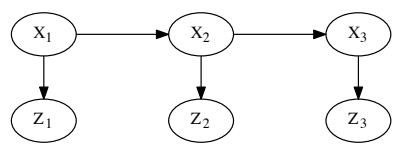
\includegraphics[width=0.45\textwidth]{factor_graph.png}}
\caption{A conceptual factor graph, adapted from \cite{10}. Poses are connected by motion factors, and landmarks by observation factors.}
\label{fig:factor_graph}
\end{figure}

The SLAM pipeline typically segregates into a front-end that handles sensor data, feature extraction, data association, and loop closure detection, and a back-end that performs global optimization. The front-end processes incoming frames, extracting constraints suitable for the back-end, which finds the configuration of poses and map points that best explains all measurements.

Loop closure is critical for large-scale mapping. As the robot travels further, incremental errors accumulate, causing drift. Detecting that the robot has revisited a known area (loop closure) introduces loop closure factors that globally correct the trajectory. Outdoors, where paths can be long and scenes partially repetitive, robust place recognition and loop closure are essential to maintain consistent global maps despite drift and environmental complexity.

Key Insights:

\begin{itemize}
    \item \textbf{Factor Graphs Exploit Sparsity:} Factor graphs allow SLAM systems to manage large maps efficiently by focusing on local interactions and maintaining global consistency through sparse connections.
    \item \textbf{Modular Front-End/Back-End Architecture:} Separating data processing from optimization facilitates the integration of diverse sensors and allows independent advancements in feature extraction and global mapping techniques.
    \item \textbf{Robust Loop Closure Mechanisms:} Effective loop closure strategies are indispensable in large-scale environments to correct drift and ensure long-term accuracy.
\end{itemize}

These foundational principles underpin all subsequent SLAM advancements. The methods discussed next build on factor graph optimization, modular front-end/back-end architectures, and robust loop closure strategies to cope with the complexities of large-scale outdoor domains.

\section{ORB-SLAM2: Efficient and Accurate Visual SLAM}
\subsection{Context and Rationale}
ORB-SLAM2 \cite{1} emerged as a benchmark in visual SLAM. Early vision-based methods often struggled to run in real-time without GPU acceleration or lacked strong global map refinements. ORB-SLAM2’s approach—efficient binary features, a triple-threaded architecture, and a reliable loop closure mechanism—set new standards for vision-based SLAM.

\subsection{Algorithmic Highlights}
\subsubsection{Fast Binary Descriptors (ORB)}
ORB (Oriented FAST and Rotated BRIEF) features are binary, rotation-invariant descriptors computed around FAST corners. They offer a good trade-off between distinctiveness and computational efficiency. Unlike heavier descriptors like SIFT or SURF, ORB features are faster to compute and match, enabling real-time performance on standard CPUs.

\subsubsection{Three-Threaded Pipeline (Tracking, Local Mapping, Loop Closing)}
ORB-SLAM2 separates tasks into three parallel threads:

\begin{itemize}
    \item \textbf{Tracking:} Estimates the camera pose for each incoming frame by matching ORB features against the local map.
    \item \textbf{Local Mapping:} Refines the local map by performing bundle adjustment on recent keyframes and adding new keyframes.
    \item \textbf{Loop Closing:} Detects when the camera revisits a previously mapped area using a bag-of-words place recognition system, and triggers global bundle adjustment to correct drift.
\end{itemize}

\subsubsection{Robust Loop Closure Detection}
ORB-SLAM2 employs a bag-of-words approach for place recognition, efficiently identifying loop closures even after traversing kilometers. Upon detecting a loop closure, it performs global bundle adjustment to align the entire trajectory, correcting accumulated drift and ensuring global map consistency.

\begin{figure}[htbp]
\centerline{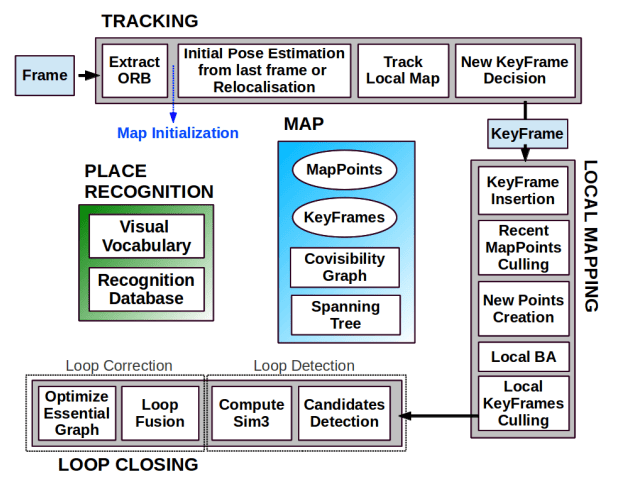
\includegraphics[width=0.45\textwidth]{orb_slam2.png}}
\caption{ORB-SLAM2 architecture diagram from \cite{1}.}
\label{fig:orb_slam2}
\end{figure}

\section{LOAM: Leveraging LiDAR for High-Fidelity Outdoor SLAM}
\subsection{Context and Motivation}
While cameras depend on illumination and texture, LiDAR sensors provide direct 3D range measurements, offering stable geometric cues regardless of lighting conditions. LOAM (Lidar Odometry and Mapping) \cite{2} demonstrated that LiDAR-based SLAM can achieve extraordinary accuracy and operate in real-time over long trajectories, making it a gold standard for autonomous driving and large-scale outdoor mapping.

\subsection{Algorithmic Highlights}
\subsubsection{Geometric Feature Selection (Edges and Planes)}
LiDAR generates dense point clouds, but processing every point is computationally expensive. LOAM extracts stable geometric primitives—sharp edges and planar surfaces—that serve as reliable references for scan matching. By focusing on these features, LOAM reduces computational load and enhances data association reliability.

\subsubsection{Decoupled Odometry and Mapping Threads}
LOAM separates the SLAM process into two main threads:

\begin{itemize}
    \item \textbf{Odometry Thread:} Runs at high frequency, aligning consecutive LiDAR scans to estimate incremental motion. It uses real-time feature matching based on extracted edges and planes.
    \item \textbf{Mapping Thread:} Operates at a lower frequency, integrating multiple scans to refine the global map and reduce drift. This thread performs more extensive optimizations, ensuring long-term map accuracy.
\end{itemize}

\subsubsection{Robust Registration Cost Functions}
LOAM minimizes geometric distances (point-to-line and point-to-plane) rather than simple point-to-point distances. This approach stabilizes optimization and accelerates convergence, as it leverages the structural stability of edges and planes.

\begin{figure}[htbp]
\centerline{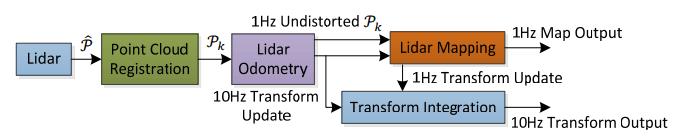
\includegraphics[width=0.45\textwidth]{loam.png}}
\caption{LOAM pipeline showing separate odometry and mapping threads from \cite{2}.}
\label{fig:loam}
\end{figure}

\section{VINS-Fusion: Multi-Sensor Integration for Enhanced Robustness}
\subsection{Context and Significance}
No single sensor modality excels under all outdoor conditions. Cameras may fail in low light or feature-poor scenes, LiDAR can be expensive or too bulky for small drones, and IMUs tend to drift over time. VINS-Fusion \cite{3} addresses these issues by tightly integrating visual and inertial data, and optionally LiDAR, into a unified factor graph framework. This multi-sensor fusion enhances robustness, adaptability, and accuracy across diverse outdoor conditions.

\subsection{Algorithmic Highlights}
\subsubsection{Tightly-Coupled Sensor Fusion in a Single Factor Graph}
VINS-Fusion combines visual keypoints, IMU preintegrated measurements, and optionally LiDAR data within the same factor graph optimization. This holistic approach ensures that all sensor constraints are considered simultaneously, leading to more accurate and stable pose estimates.

\subsubsection{IMU Preintegration for Efficiency}
Handling high-frequency IMU data directly would be computationally prohibitive. VINS-Fusion employs an IMU preintegration technique that summarizes multiple IMU readings between keyframes into a single factor. This approach preserves essential motion information while reducing the computational burden.

\subsubsection{Optional Integration of LiDAR Data}
VINS-Fusion’s framework is extensible, allowing the integration of LiDAR data alongside visual and inertial measurements. This optional inclusion further enhances scale accuracy and stability, especially in environments where visual features are sparse or unreliable.

\begin{figure}[htbp]
\centerline{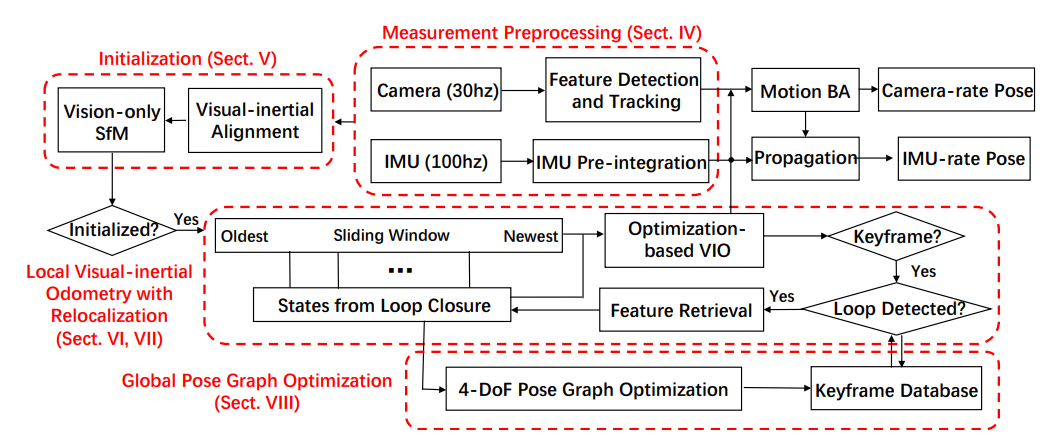
\includegraphics[width=0.45\textwidth]{vins_fusion.png}}
\caption{VINS-Fusion factor graph integration of multiple sensors from \cite{3}.}
\label{fig:vins_fusion}
\end{figure}

\section{Advanced Frontiers: Direct Methods, Semantic Understanding, and Learning-Based Enhancements}
Building upon the foundational algorithms, the SLAM community has explored advanced techniques to tackle specific outdoor challenges: low-texture regions, dynamic objects, and environmental variability. We delve into direct visual methods, semantic SLAM, and learning-based approaches that offer complementary strengths and address limitations of earlier systems.

\subsection{Direct Visual Methods: LSD-SLAM and DSO}
Direct methods for SLAM bypass traditional feature extraction, instead optimizing camera poses directly against pixel intensities. LSD-SLAM \cite{4} and Direct Sparse Odometry (DSO) \cite{5} exemplify this approach, offering benefits in low-texture environments but facing challenges with illumination changes.

\subsubsection{Photometric Error Minimization}
Unlike feature-based SLAM, direct methods minimize the photometric error between images by aligning pixel intensities. This allows them to utilize subtle intensity gradients that feature detectors might miss, enabling better performance in texture-poor or repetitive environments.

\subsubsection{Semi-Dense or Dense Mapping}
Direct methods typically produce semi-dense or dense reconstructions, capturing more geometric detail than sparse feature-based methods. This richer map can aid in tasks like obstacle avoidance and terrain understanding, which are crucial for autonomous navigation in complex outdoor terrains.

\subsubsection{Handling Illumination Changes}
Direct methods are inherently more sensitive to lighting variations since they rely on consistent pixel intensities. Techniques like robust photometric error models, image normalization, and adaptive brightness adjustments are employed to mitigate these issues.

\begin{figure}[htbp]
\centerline{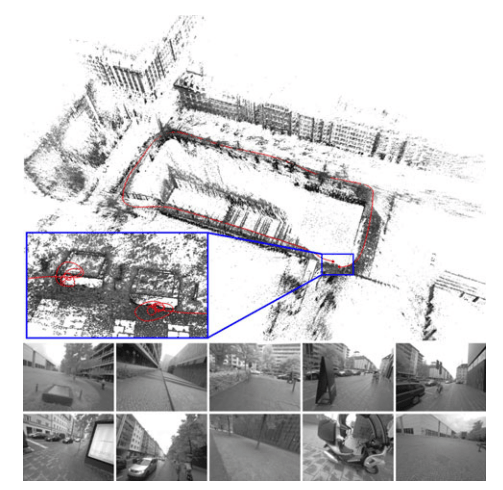
\includegraphics[width=0.45\textwidth]{dso.png}}
\caption{DSO’s semi-dense reconstruction from \cite{5}.}
\label{fig:dso}
\end{figure}

\subsection{Semantic and Dynamic-Scene SLAM: DynaSLAM}
Outdoor environments are inherently dynamic, with moving objects such as pedestrians, vehicles, and animals. DynaSLAM \cite{6} integrates semantic segmentation to identify and exclude dynamic elements from the SLAM process, thereby enhancing map stability and accuracy.

\subsubsection{Semantic Segmentation for Dynamic Filtering}
DynaSLAM employs a deep neural network (e.g., Mask R-CNN) to classify image pixels into semantic categories. By identifying and masking out dynamic objects like cars and people, it ensures that only static elements contribute to the SLAM optimization.

\subsubsection{Enhanced Loop Closure and Map Consistency}
By excluding dynamic objects, DynaSLAM reduces the likelihood of false loop closures and ensures that loop detection relies on stable landmarks. This leads to more reliable global optimization and a consistent global map over extended trajectories.

\begin{figure}[htbp]
\centerline{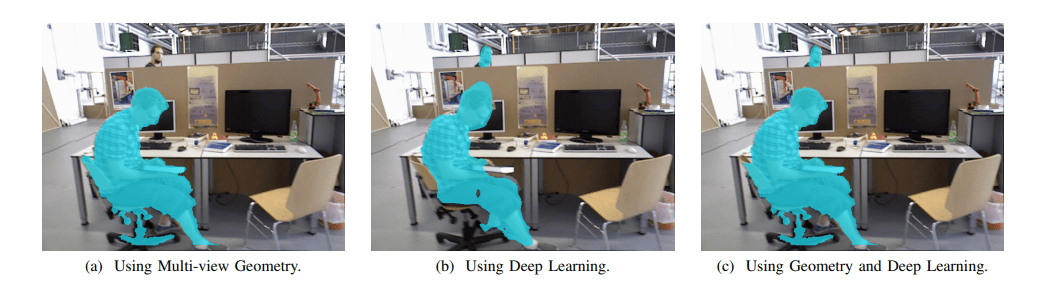
\includegraphics[width=0.45\textwidth]{dynaslam.png}}
\caption{DynaSLAM’s semantic segmentation filtering out dynamic objects from \cite{6}.}
\label{fig:dynaslam}
\end{figure}

\subsection{Learning-Based Approaches: SuperGlue and DeepVO}
The integration of deep learning into SLAM front-ends has opened new avenues for enhancing feature matching and motion estimation. SuperGlue \cite{7} and DeepVO \cite{8} leverage neural networks to improve robustness and adaptability in diverse outdoor conditions.

\subsubsection{Learned Feature Matching (SuperGlue)}
SuperGlue uses a graph neural network to perform feature matching between image pairs, considering the spatial and contextual relationships of features. This approach goes beyond traditional nearest-neighbor matching by enforcing mutual consistency and global coherence in correspondences.

\subsubsection{End-to-End Motion Estimation (DeepVO)}
DeepVO trains a deep neural network to predict camera motion directly from raw image sequences. By learning from large datasets, it can implicitly capture complex motion patterns and environmental cues, offering an alternative to traditional geometric motion estimation.

\section{Comparative Analysis of Selected Approaches}
To synthesize the insights, we present a comparative table summarizing the key characteristics of selected state-of-the-art SLAM methods. This table highlights their sensors, core strategies, strengths, limitations, and suitability for outdoor applications.

\begin{table}[htbp]
\caption{Comparative Overview of Representative SLAM Methods}
\begin{center}
\begin{adjustbox}{width=\columnwidth,center}
\begin{tabular}{|p{1.5cm}|p{1.3cm}|p{2.3cm}|p{1.5cm}|p{1.5cm}|}
\hline
\textbf{Method} & \textbf{Sensors} & \textbf{Core Idea} & \textbf{Strengths} & \textbf{Limitations} \\
\hline
ORB-SLAM2 \cite{1} & Camera & Binary features, loop closure & Real-time, accurate & Low-texture/lighting \\
\hline
LOAM \cite{2} & LiDAR & Geometric features, decoupled threads & High accuracy & High cost, complex \\
\hline
VINS-Fusion \cite{3} & Cam + IMU (+LiDAR) & Multi-sensor fusion & Robust, adaptable & High complexity \\
\hline
LSD-SLAM \cite{4}, DSO \cite{5} & Camera & Direct photometric opt. & Low-texture areas & Sensitive to lighting \\
\hline
DynaSLAM \cite{6} & Cam (+Semantic) & Semantic filtering & Dynamic scenes & GPU req., training \\
\hline
SuperGlue \cite{7} & Cam (Learned) & Learned matching (GNN) & Improved matches & NN cost, training data \\
\hline
DeepVO \cite{8} & Cam (Learned) & End-to-end odometry & Adaptive & Large dataset req. \\
\hline
\end{tabular}
\end{adjustbox}
\label{tab:comparison}
\end{center}
\end{table}

\section{Persistent Challenges and Future Directions}
Despite significant advancements, several enduring challenges remain for large-scale outdoor SLAM:

\subsection{Dynamic Scenes and Predictive Modeling}
Current semantic methods, such as DynaSLAM, primarily filter out dynamic objects. Future research may incorporate predictive models that anticipate object movements, integrating dynamic element trajectories into the SLAM process. This proactive approach could enhance map stability and provide richer environmental understanding.

\subsection{Lifelong Operation and Seasonal Adaptation}
Outdoor environments are not static. Vegetation grows or sheds leaves, buildings are constructed or demolished, and weather patterns change. Kimera \cite{11} addresses some of these issues by integrating metric-semantic localization, but continual adaptation remains a challenge. Lifelong SLAM systems must continuously update maps, discard obsolete information, and incorporate new data without restarting the mapping process. Techniques like incremental learning and domain adaptation are essential to maintain long-term accuracy and relevance.

\subsection{Weather and Illumination Invariance}
Outdoor SLAM systems must cope with a wide range of weather conditions and lighting scenarios. Heavy rain, fog, snow, or nighttime darkness can degrade sensor performance. Integrating additional sensors like radar or thermal cameras can provide resilience against such conditions. Learning-based methods can also be trained to adapt to varying domains, enhancing SLAM’s robustness to environmental changes.

\subsection{Scalability in Factor Graph Optimization}
As SLAM systems operate over longer trajectories, the size of the factor graph increases, posing computational challenges. Hierarchical SLAM architectures that break down the environment into manageable submaps, along with incremental optimization techniques, can help maintain real-time performance. Emerging optimization paradigms, such as distributed or parallel computing, and hardware accelerations like GPUs or specialized processors, may further enhance scalability.

\subsection{Integration of Novel Sensors and Modalities}
The advent of new sensor technologies, such as event cameras, thermal imaging, or advanced radar systems, offers opportunities to enhance SLAM. Integrating these sensors into existing frameworks requires adaptable front-ends and new factor definitions within factor graphs. The modularity of frameworks like VINS-Fusion facilitates such integrations, paving the way for more versatile and capable SLAM systems.

\subsection{Unified Scene Understanding and Task-Level Integration}
Future SLAM systems may need to integrate higher-level scene understanding and task-specific information. For instance, agricultural robots might prioritize crop features, while delivery drones focus on navigational landmarks. Integrating semantic reasoning and task objectives can make SLAM not only about mapping and localization but also about understanding and interacting with the environment in meaningful ways.

\subsection{Hybrid and Learned Optimization Approaches}
Combining classical optimization with learned models could yield faster, more accurate SLAM systems. For example, learned components could provide initial pose estimates or guide loop closure detection, while classical optimizers ensure global consistency. Reinforcement learning might be used to develop exploration strategies that maximize map informativeness, enhancing overall SLAM performance in unknown environments.

\subsection{Benchmarks and Standardization}
While datasets like KITTI \cite{12} and EuRoC MAV \cite{13} have driven SLAM research, more comprehensive benchmarks capturing a wider range of outdoor conditions are needed. These benchmarks should include diverse weather, lighting, and dynamic scenarios to evaluate SLAM systems’ robustness and generalization capabilities accurately.

\section{Conclusion}
SLAM has matured from a niche research area focused on small indoor spaces to a critical technology enabling autonomous navigation in complex, large-scale outdoor environments. This evolution has been driven by foundational insights into factor graph optimization, modular front-end/back-end architectures, and robust loop closure mechanisms, as exemplified by canonical systems like ORB-SLAM2, LOAM, and VINS-Fusion.

Building on these foundations, advanced techniques have addressed specific outdoor challenges: direct visual methods exploit pixel intensities to handle low-texture areas, semantic SLAM integrates scene understanding to manage dynamic objects, and learning-based approaches enhance feature matching and motion estimation through neural networks. These innovations demonstrate the field’s adaptability and the importance of integrating diverse algorithmic strategies to achieve robust, scalable SLAM.

Despite significant progress, large-scale outdoor SLAM continues to grapple with challenges such as dynamic scenes, environmental variability, scalability, and the integration of novel sensors and semantics. Addressing these issues will require ongoing research into predictive dynamic modeling, lifelong adaptability, multi-modal sensor fusion, scalable optimization algorithms, and semantic reasoning within SLAM frameworks.

As the demand for autonomous systems in outdoor environments grows—ranging from self-driving cars and delivery drones to agricultural robots and exploration rovers—the lessons gleaned from current state-of-the-art SLAM methods will guide the development of next-generation solutions. These future SLAM systems will be more resilient, adaptable, and intelligent, capable of navigating and mapping the vast, dynamic, and ever-changing real world with unprecedented reliability and efficiency.

\begin{thebibliography}{00}
\bibitem{1} R. Mur-Artal, J. Montiel, and J.D. Tardós, “ORB-SLAM: A versatile and accurate monocular SLAM system,” IEEE Transactions on Robotics, 31(5):1147–1163, 2015.
\bibitem{2} J. Zhang and S. Singh, “LOAM: Lidar Odometry and Mapping in Real-time,” Robotics: Science and Systems (RSS), 2014.
\bibitem{3} T. Qin, P. Li, and S. Shen, “VINS-Fusion: A versatile and robust multi-sensor fusion framework for visual-inertial state estimation,” IEEE Transactions on Robotics, 34(4):1004–1020, 2018.
\bibitem{4} J. Engel, T. Schöps, and D. Cremers, “LSD-SLAM: Large-scale direct monocular SLAM,” European Conference on Computer Vision (ECCV), 2014.
\bibitem{5} J. Engel, V. Koltun, and D. Cremers, “Direct Sparse Odometry,” IEEE Transactions on Pattern Analysis and Machine Intelligence, 40(3):611–625, 2018.
\bibitem{6} B. Bescós, J. Neira, R. Mur-Artal, and J.D. Tardós, “DynaSLAM: Tracking, mapping, and inpainting in dynamic scenes,” IEEE Transactions on Robotics, 36(6):2032–2038, 2020.
\bibitem{7} P. Sarlin, D. DeTone, T. Malisiewicz, and A. Rabinovich, “SuperGlue: Learning feature matching with graph neural networks,” Conference on Computer Vision and Pattern Recognition (CVPR), 2020.
\bibitem{8} S. Wang, R. Clark, H. Wen, and N. Trigoni, “DeepVO: Towards end-to-end visual odometry with deep recurrent convolutional neural networks,” IEEE International Conference on Robotics and Automation (ICRA), 2017.
\bibitem{9} G. Klein and D. Murray, “Parallel tracking and mapping for small AR workspaces,” International Symposium on Mixed and Augmented Reality (ISMAR), 2007.
\bibitem{10} F. Dellaert, “Factor Graphs and GTSAM: A hands-on introduction,” Technical Report, 2012.
\bibitem{11} A. Rosinol, M. Abate, Y. Chang, and L. Carlone, “Kimera: an open-source library for real-time metric-semantic localization and mapping,” IEEE International Conference on Robotics and Automation (ICRA), 2020.
\bibitem{12} A. Geiger, P. Lenz, and R. Urtasun, “Are we ready for autonomous driving? The KITTI vision benchmark suite,” Conference on Computer Vision and Pattern Recognition (CVPR), 2012.
\bibitem{13} R. Kümmerle et al., “g2o: A general framework for graph optimization,” IEEE International Conference on Robotics and Automation (ICRA), 2011.
\bibitem{14} J.T. Barron, B. DeTone, A. Dusmanu, and C. Sweeney, “CodeSLAM: Learning a Compact, Optimisable Representation for Dense Visual SLAM,” Conference on Computer Vision and Pattern Recognition (CVPR), 2018.
\bibitem{15} Z. Zhi, J. Dong, K. Guo, M. Gharbi, T. Funkhouser, and Q. Huang, “NICE-SLAM: Neural Implicit Scalable Encoding for SLAM,” Conference on Computer Vision and Pattern Recognition (CVPR), 2022.
\end{thebibliography}

\end{document}